\documentclass[11pt,landscape]{article}
\usepackage{multicol}
\usepackage{calc}
\usepackage{ifthen}
\usepackage[landscape]{geometry}
\usepackage{hyperref}
\usepackage{lipsum}  

\ifthenelse{\lengthtest { \paperwidth = 11in}}
	{ \geometry{top=.5in,left=.5in,right=.5in,bottom=.5in} }
	{\ifthenelse{ \lengthtest{ \paperwidth = 297mm}}
		{\geometry{top=1cm,left=1cm,right=1cm,bottom=1cm} }
		{\geometry{top=1cm,left=1cm,right=1cm,bottom=1cm} }
	}

% Turn off header and footer
\pagestyle{empty}
 \usepackage{amsmath}

% Redefine section commands to use less space
\makeatletter
\renewcommand{\section}{\@startsection{section}{1}{0mm}%
                                {-1ex plus -.5ex minus -.2ex}%
                                {0.5ex plus .2ex}%x
                                {\normalfont\large\bfseries}}
\renewcommand{\subsection}{\@startsection{subsection}{2}{0mm}%
                                {-1explus -.5ex minus -.2ex}%
                                {0.5ex plus .2ex}%
                                {\normalfont\normalsize\bfseries}}
\renewcommand{\subsubsection}{\@startsection{subsubsection}{3}{0mm}%
                                {-1ex plus -.5ex minus -.2ex}%
                                {1ex plus .2ex}%
                                {\normalfont\small\bfseries}}
\makeatother

% Define BibTeX command
\def\BibTeX{{\rm B\kern-.05em{\sc i\kern-.025em b}\kern-.08em
    T\kern-.1667em\lower.7ex\hbox{E}\kern-.125emX}}

% Don't print section numbers
\setcounter{secnumdepth}{0}
\usepackage{circuitikz}


\setlength{\parindent}{0pt}
\setlength{\parskip}{0pt plus 0.5ex}
\usepackage{karnaugh-map}


% -----------------------------------------------------------------------

\begin{document}

\raggedright
\footnotesize
\begin{multicols}{3}


% multicol parameters
% These lengths are set only within the two main columns
%\setlength{\columnseprule}{0.25pt}
\setlength{\premulticols}{1pt}
\setlength{\postmulticols}{1pt}
\setlength{\multicolsep}{1pt}
\setlength{\columnsep}{2pt}

\begin{center}
     \Large{\textbf{ECE253 Midterm Cheatsheet}} \\
\end{center}



\section{Boolean Algebra}
\textbf{De Morgan's Theorem} tells us
\begin{equation}
    \overline{x\cdot y}=\overline{x}+\overline{y}, \quad\quad\quad \overline{x+y}=\overline{x}\cdot\overline{y}
\end{equation}
Inverting the inputs to an \verb!or! gate is the same as inverting the outputs to an \verb!and! gate, and the other way around. We also have: 
\begin{itemize}
    \item $(x+y)(y+z)(\overline{x}+z)=(x+y)(\overline{x}+z)$
    \item $x+yz=(x+y)(x+z)$
    \item $x+xy=x$ (Absorption)
    \item $xy+x\overline{y}=x$ (Combining)
    \item $(x+y)(x+\overline{y})=x$
    \item $ x+\overline{x}y=x+y$
    \item $x(\overline{x}+y)=xy$
    \item $xy+yz+z\overline{x}=xy+z\overline{x}$ (Consensus)
\end{itemize}

\subsection{Gates}
\begin{center}
    \begin{tabular}{c|c||c|c||c|c}
        \verb!AND! & \begin{circuitikz}[scale=0.7, transform shape] 
            \draw(0,0) node[and port] {};
        \end{circuitikz} & 

        \verb!OR! & \begin{circuitikz}[scale=0.7, transform shape] 
            \draw(0,0) node[or port] {};
        \end{circuitikz} &
        \verb!NOT! & \begin{circuitikz}[scale=0.7, transform shape] 
            \draw(0,0) node[not port] {};
        \end{circuitikz} \\ \hline
        \verb!NOR! & \begin{circuitikz}[scale=0.7, transform shape] 
            \draw(0,0) node[nor port] {};
        \end{circuitikz} &
        \verb!NAND! & \begin{circuitikz}[scale=0.7, transform shape] 
            \draw(0,0) node[nand port] {};
        \end{circuitikz} &
        \verb!XOR! & \begin{circuitikz}[scale=0.7, transform shape] 
            \draw(0,0) node[xor port] {};
        \end{circuitikz}
    \end{tabular}
\end{center}
\subsection{SOPs and POSs}
We can create boolean algebra expressions for truth tables.
\vspace{2mm}

\textbf{Minterm:} Corresponds to each row of truth table, i.e. $m_3=\overline{x_2}x_1x_0$ such that when $3=0b011$ is substituted in, $m_3=1$ and $m_3=0$ otherwise.  

\textbf{Maxterm:} They give $M_i=0$ if and only if the input is $i$. For example, $M_3=x_2+\overline{x_1}+\overline{x_0}.$

\textbf{SOP and POS:} Truth tables can be represented as a sum of minterms, or product of maxterms.
\begin{itemize}
    \item Use minterms when you have to use \verb!NAND! gates and maxterms when you have to use \verb!NOR! gates.
    \item When converting expressions to its dual, it's often helpful to negate expressions twice, or draw out the logic circuit.
\end{itemize}
\subsection{Cost}
The cost of a logic circuit is given by
\begin{equation}
    \text{cost} = \text{gates} + \text{inputs}
\end{equation}
If an inversion (\verb!NOT!) is performed on the primary inputs, then it is not included. If it is needed inside the circuit, then the \verb!NOT! gate is included in the cost.
\subsection{Karnaugh Map}
Method of finding a minimum cost expression: We can map out truth table on a grid for easier pattern recognition. Example of a four variable map is shown below:
\begin{center}
    \begin{karnaugh-map}[4][4][1][$x_2x_1$][$x_4x_3$]
        \minterms{0,1,3,4,5,7,11,14,15,10}
        \maxterms{2,6,8,9,10,12,13}
        % \indeterminants{2,5}
        \implicant{0}{5}
        \implicant{3}{11}
        \implicant{15}{10}
        % \implicant{4}{5}
    \end{karnaugh-map}
\end{center}
\vspace{-8mm}
and the representation is $\overline{x_2}\cdot\overline{x_4}+x_2 \cdot x_1+\overline{x_4} \cdot x_2$ when using \textit{minterms}. To use \textit{maxterms}, we take the intersection of sets that don't include blocks of $0$s. For example, $(\overline{x_2}\cdot \overline{x_1})(\overline{x_2}+x_1+x_4).$ Some \textit{rules}: 
\begin{itemize}
    \item Side lengths should be powers of $2$ and be as large as possible.
    \item Use \textbf{graycoding}: adjacent rows/columns should share one bit.
\end{itemize}
Some \textit{definitions:}
\begin{itemize}
    \item \textbf{Literal:} variables in a product term: $x_1\overline{x_2}x_3$ has three literals.
    \item \textbf{Implicant:} a product term that indicates the input valuation(s) for which a given function is equal to $1$.
    \item \textbf{Prime Implicant:} an implicant that cannot be combined into another implicant with fewer literals. \textit{They are as big as possible.}
    \item \textbf{Cover:} A collection of implicants that account for all valuations for which function equals $1$.
    \item \textbf{Essential Prime Implicant:} A prime implicant that includes a minterm not included in any other prime implicant. \textit{They contain at least one minterm not covered by another prime implicant.}
\end{itemize}
In the above example, $\overline{x_2}\cdot \overline{x_4}+x_2x_1+\overline{x_4}x_2$ are prime implicants.

\subsubsection{Minimization Procedure}
\begin{enumerate}
    \item Generate all prime implicants for given function $f$
    \item Find the set of essential prime implicants
    \item Determine the nonessential prime implicants that should be added.
\end{enumerate}
\subsection{Common Logic Gates}
To save space, boolean expressions will be written instead of drawing diagrams. You should be familiar with how to construct diagrams from expressions.
\begin{itemize}
    \item \textbf{Mux 2$\rightarrow$1:} $\verb#mux2to1#(s,x_0,x_1) = \overline{s}x_0+sx_1$
    \item \textbf{Mux 4$\rightarrow$1:} $\verb#mux4to1#(s,x) = \verb#mux2to1#\left(s1,\verb#mux2to1#(s0,x0,x1),\verb#mux2to1#(s0,x2,x3)\right)$
    \item \textbf{Not:} \verb#not(x)=nand(x,x)=nor(x,x)#
    \item \verb!XOR! acts as modular arithmetic.
    \item Multiplexers are functionally complete. $\verb!AND!=mux(x,y,1)$, $\verb!OR!=mux(x,0,y).$
\end{itemize}
\subsection{RS Latch}
Sequential circuits depend on sequence of inputs. A \textbf{SR Latch} are cross-coupled \verb!NOR! gates.
\vspace{2mm}
% \begin{center}
    {
    \begin{multicols}{2}
        \begin{center}
            \begin{circuitikz} \draw
                (0,2) node[nor port] (NOR1) {}
                (1,2) node[anchor=east] {Q}
                (1,0) node[anchor=east] {$\overline{Q}$}
                (0,0) node[nor port] (NOR2) {}
                (NOR1.in 1) node[anchor=east] {R}
                (NOR2.in 2) node[anchor=east] {S}
                (NOR1.out) -- ++(0,-0.5) -- ($(NOR2.in 1) +(0,0.5)$) -- (NOR2.in 1)
                (NOR2.out) -- ++(0,+0.5) -- ($(NOR1.in 2) +(0,-0.5)$)--(NOR1.in 2)
                ;\end{circuitikz}
        \end{center}


        \begin{center}
            \begin{tabular}{c|c|c|c}
                S & R & Q & $\overline{Q}$ \\ \hline
                0 & 0 & 0/1 & 1/0 \\
                0 & 1 & 0 & 1 \\ 
                1 & 0 & 1 & 0 \\ 
                1 & 1 & 0 & 0
           \end{tabular}
        \end{center}
        \vspace{-2mm}
        \scriptsize When $S=R=0$, it stores the last $Q$ value. In practice, we should not have $S=R=1$.
    \end{multicols}
}
\subsection{Gated D Latch and Clock Signal}
{
    \begin{multicols}{2}
        \begin{center}
            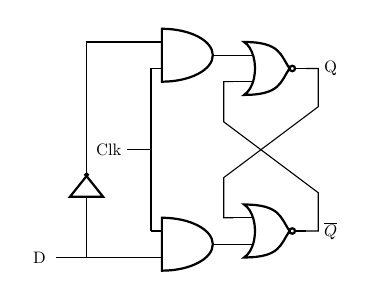
\begin{tikzpicture}[scale=0.6, transform shape]
 
                % Draw and gates
                \node[and port] (and1) at (0,2) {};
                \node[and port] (and2) at (0,-2) {};
                 
                % Draw nor gates
                \draw (and1.out) -- ++(0.2,0) node
                [
                    nor port,
                    anchor=in 1
                ] (nor1) {};
                 
                \draw (and2.out) -- ++(0.2,0) node
                [
                    nor port,
                    anchor=in 2
                ] (nor2) {};
                 
                \draw (nor1.in 2) -| ++ (-0.2,-0.85) -- ++(2,-1.5) coordinate(a) |- (nor2.out);
                \draw (nor2.in 1) -| ++ (-0.2,0.85) -- ++(2,1.5) |- (nor1.out);
                 
                % Clock
                \draw (and1.in 2) -- (and2.in 1)node[midway](clk){};
                \draw (clk.center) -- ++(-0.5,0) node[left]{Clk};
                 
                % Output labels
                \draw (nor1.out -| a) node[right]{Q};
                \draw (nor2.out -| a) node[right]{$\overline{Q}$};
                 
                \draw (and2.in 2) -- ++(-2,0) coordinate(a2) node[left=0.1cm]{D};
                 
                % Not port
                \node
                [
                    not port,
                    rotate=90,
                    scale=0.5,
                ](not) at (-2.75,-0.75){};
                 
                \draw (not.in) |- (a2) (not.out) |- (and1.in 1)  ;
                 
                \end{tikzpicture}
        \end{center}


        \begin{center}
            \begin{tabular}{c|c|c}
                Clk & D & $Q(t+1)$ \\ \hline
                0 & x & Q(t) \\
                1 & 0 & D
           \end{tabular}
        \end{center}
        \vspace{-3mm}
        \scriptsize Where the $\text{Clk}=1$ cases refer to \verb!retain!, \verb!reset!, \verb!set!, and last one is not used.
    \end{multicols}
}

% \end{center}
\subsection{D Flip Flops}
Consists of two gated D latches, connected in series and both connected to the same clock. However, clock input for the first D latch is inverted.
\begin{itemize}
    \item When the clock rises up, $Q$ stores value of $D$.
\end{itemize}
\textbf{Registers:} Multiple flip flops connected together.
\end{multicols}
\begin{multicols*}{3}
\subsection{Verilog}
\subsubsection{Logic Operators}
\begin{center}
    \begin{tabular}{c|c||c|c}
        \verb!bitwise AND! & \verb!&! &
        \verb!bitwise OR! & \verb!|! \\ \hline
        \verb!bitwise NAND! & \verb!~&! &
        \verb!bitwise NOR! & \verb!~!!  \\ \hline
        \verb!bitwise XOR! & \verb!^! &
        \verb!bitwise XNOR! & \verb!~^! \\ \hline
        \verb!logical negation! & \verb!!! &
        \verb!bitwise negation! & \verb!~! \\ \hline 
        \verb!concatenation! & \verb!{}! &
        \verb!replication! & \verb!{{}}! 
    \end{tabular}
\end{center}
\begin{itemize}
    \item \verb!reduction! operators are put at the start and output a scalar.
    \item \verb!bitwise! operators 
    \item \verb!blocking assignment =!: executed in the order they are specified.
    \item\verb!Nonblock assignments <=! executed in parallel.
\end{itemize}

\subsubsection{Minimal Example}
\begin{verbatim}
module mux(MuxSelect, Input, Out);
    input [4:0] Input; input [2:0] MuxSelect;
    output Out;
    reg Out; // declare output for always block
    always @(*) // declare always block
    	begin
    	case (MuxSelect[2:0]) // start case statement
    	3'b000: Out = Input[0]; // case 0
    	3'b001: Out = Input[1]; // case 1
    	3'b010: Out = Input[2]; // case 2
    	3'b011: Out = Input[3]; // case 3
    	3'b100: Out = Input[4]; // case 4
    	default: Out = 1'bx; // default case
    	endcase
    end
endmodule
\end{verbatim}
\subsubsection{Half Adder}
\begin{verbatim}
module HA(x, y, s, c);
    input x, y; output s, c;
    assign s = x^y;
    assign c = x&y;
endmodule
\end{verbatim}
\subsubsection{Full Adder}
\begin{verbatim}
module FA(a, b, c_in, s_out, c_out);
    input a, b, c_in; output s_out, c_out;
    wire w1, w2, w3;
    HA u0(.x(a), .y(b), .s(w1), .c(w2));
    HA u1(.x(c_in), .y(w1), .s(s_out), .c(w3));
    assign c_out = w2|w3;
endmodule
\end{verbatim}
\subsubsection{D Latch}
\begin{verbatim}
module D-latch(D, clk, Q);
    input D, clk;
    output reg Q;
    always@(D, clk)
    begin
        if (clk == 1'b1) Q = D;
    end
endmodule
\end{verbatim}
\subsection{Flip Flop}
\begin{verbatim}
module D-ff(D, clk, Q);
    input D, clk;
    output reg Q;   
    always@(posedge clk) Q <= D; // use <= operator
endmodule
\end{verbatim}
\subsection{Flip Flop (stores on both edges)}
\begin{verbatim}
module DDR (input c, input D, output Q) ;
    reg p, n;
    always @ (posedge c) p <= D;
    always @ (negedge c) n <= D;
    assign Q <= c ? p : n;
endmodule
\end{verbatim}
\subsection{Registers}
\begin{verbatim}
module reg8(D, clk, Q);
    input clock;
    input [7:0] D;
    output reg[7:0] Q;
    always@(posedge clock)
        Q <= D;
    endmodule
\end{verbatim}
\subsection{ModelSim Do Files}
\begin{verbatim}
# set working dir, where compiled verilog goes
vlib work
# compile all verilog modules in mux.v to working
# dir could also have multiple verilog files
vlog mux.v
#load simulation using mux as the
# top level simulation module
vsim mux
#log all signals and add some signals to
# waveform window
log {/*}
# add wave {/*} would add all items in
# top level simulation module
add wave {/*}
# first test case
#set input values using the force command
# signal names need to be in {} brackets
force {SW[0]} 0
force {SW[1]} 0
force {SW[9]} 0
run 10ns
\end{verbatim}
\textbf{ModelSim and Other Lab Things}
\begin{itemize}
    \item FGPA: Field Programmable Gate Array
    \item To repeat signals, use this syntax: 
    \begin{verbatim}
    force {MuxSelect[2]} 0 0ns, 1 {4ns} -r 8ns
    \end{verbatim}
    \vspace{-4mm}
    which starts at $0$ at 0ns, $1$ at 4ns, and repeats every $8$ ns.
    \item On the \verb!DE1-SoC! board, hex thing is red if $0$ and white if $1$.
\end{itemize}
\subsection{Frequency Dividers}
\begin{itemize}
    \item To half the frequency, connect $\overline{Q}$ to $D$ on the same gated D latch.
    \item To quarter the frequency, connect $\overline{Q}$ to the clock of the next gated D latch (which is set up the same as the half frequency case).
    \item To reduce frequency by $2k$, connect $k$ D latches connected in series ($D$ to $Q$) and to the same clock. First $D$ is connected to last $\bar{Q}$. The last $Q$ will have a reduced frequency of $2k$.
\end{itemize}
\subsection{Add Extra Things Below}

\end{multicols*}
\end{document}
